\documentclass[11pt,a4paper,openright,twoside]{article}
\usepackage[english]{babel}
\usepackage{newlfont}
\usepackage{color}
\textwidth=450pt\oddsidemargin=0pt
\usepackage{graphicx}
\usepackage{float}
\usepackage{textcomp}
\usepackage{caption}
\usepackage{wrapfig}
\usepackage{subfig}
\usepackage{sidecap}
\usepackage[rlft]{floatflt}
\usepackage{amsmath}
\usepackage{amssymb}
\usepackage{bm}
\usepackage{fancyhdr}
\usepackage{multirow}
\usepackage[utf8x]{inputenc}
\usepackage{fullpage}
\usepackage[Lenny]{fncychap}
\usepackage[T1]{fontenc}
\usepackage[normalem]{ulem}
\usepackage{booktabs}
\usepackage{enumerate}

\usepackage[usenames,dvipsnames]{xcolor}
\usepackage{listings}
\usepackage{xcolor}

\definecolor{light-gray}{gray}{0.95}
\lstset{language=R,
    basicstyle=\small\ttfamily,
    stringstyle=\itshape\color{RedViolet},
    showstringspaces=false,
    otherkeywords={0,1,2,3,4,5,6,7,8,9},
    morekeywords={TRUE,FALSE, ggplot, data.frame, theme, ylab, xlab},
    deletekeywords={data, frame, beta, c, par, colours, contour, scale,
                    panel, grid, hat},
    keywordstyle=\color{RoyalBlue},
    commentstyle=\itshape\color{PineGreen},
    backgroundcolor=\color{light-gray}
}

\title{CTRP - A Toy Example}
\author{}
\date{}





\begin{document}

\maketitle


\section{Data.} We simulate a covariate matrix $\mathbf{X}$ having $n=20$ observations of $f=5$ variables from a standard normal distribution. Then we simulate a response variable $\mathbf{y}=(y_1,\ldots,y_n)^\top$ according to the logistic regression model
\begin{align*}
y_j\sim\text{Ber}(p_j),\quad\quad\text{logit}(p_j)=\beta_0+\mathbf{X}_j\boldsymbol{\beta}\quad\quad(j=1,\ldots,n)
\end{align*}
with $\beta_0=0$ and $\mathbf{\beta}=(20,10,5,0,0)$.

Finally, we consider $B$ random permutations of $\mathbf{y}$ (where the first is the identity) and compute the global test statistics
\begin{align*}
g_i^\pi =\mathbf{y}^{\pi\top}\left(\mathbf{I}-\frac{1}{n}\mathbf{1}\mathbf{1}^\top\right)\mathbf{X}_i\mathbf{X}_i^\top\left(\mathbf{I}-\frac{1}{n}\mathbf{1}\mathbf{1}^\top\right)\mathbf{y}^{\pi} \quad\quad(i=1,\ldots,f,\quad \pi=1,\ldots,B),
\end{align*}
as well as the centered test statistics
\begin{align*}
d_i^\pi=g_i^\pi - g_i\quad\quad(i=1,\ldots,f,\quad \pi=1,\ldots,B).
\end{align*}

We define the matrix $M$ of the individual centered test statistics $d_i^\pi$, where the rows are sorted so that the observed values $g_i$ are in increasing order, as well as the matrix $D$, obtained by sorting the elements of $M$ within each row in descending order:
\begin{table}[h!]
\centering
\resizebox{\textwidth}{!}{
\begin{tabular}{ccccccccccc}
\multicolumn{5}{c}{$\mathbf{M}$} & & \multicolumn{5}{c}{$\mathbf{D}$}\\
$d_5$ & $d_2$ & $d_3$ & $d_4$ & $d_1$ &  &  &  &  &  &  \\
\cline{1-5} \cline{7-11}
0.00 & 0.00 & 0.00 & 0.00 & 0.00 &  & 0.00 (1)& 0.00 (4)& 0.00 (3)& 0.00 (2)& 0.00 (5)\\
-6.03 & -7.99 & -8.84 & -16.62 & -28.32 &  & -6.03 (5)& -7.99 (2)& -8.84 (3)& -16.62 (4)& -28.32 (1)\\
-5.29 & -5.02 & -9.04 & -13.61 & -27.72 &  & -5.02 (2)& -5.29 (5)& -9.04 (3)& -13.61 (4)& -27.72 (1)\\
2.43 & -8.25 & -9.14 & 13.63 & -27.34 &  & 13.63 (4)& 2.43 (5)& -8.25 (2)& -9.14 (3)& -27.34 (1)\\
-5.63 & -6.49 & -8.38 & -9.23 & -28.19 &  & -5.63 (5)& -6.49 (2)& -8.38 (3)& -9.23 (4)& -28.19 (1)\\
-6.08 & -6.51 & -9.38 & -16.64 & -26.59 &  & -6.08 (5)& -6.51 (2)& -9.38 (3)& -16.64 (4)& -26.59 (1)\\
-4.59 & -3.36 & -8.34 & -14.86 & -10.74 &  & -3.36 (2)& -4.59 (5)& -8.34 (3)& -10.74 (1)& -14.86 (4)\\
-5.85 & -9.07 & -5.33 & 9.44 & -26.65 &  & 9.44 (4)& -5.33 (3)& -5.85 (5)& -9.07 (2)& -26.65 (1)\\
-0.28 & -0.89 & -4.98 & -16.31 & -25.71 &  & -0.28 (5)& -0.89 (2)& -4.98 (3)& -16.31 (4)& -25.71 (1)\\
2.72 & 14.70 & -6.99 & -16.65 & -27.27 &  & 14.70 (2)& 2.72 (5)& -6.99 (3)& -16.65 (4) & -27.27 (1)
\end{tabular}
}
\end{table}



\newpage
\section{Test.} Assume that we want to test $S=\{3\}$. Then the subsets that need to be tested are the following:

\begin{table}[h!]
\centering
\resizebox{\textwidth}{!}{
\begin{tabular}{c|ccccccccccc}
size &   &  &  &  &  &  &  &  &  &  &  \\
5 &  &  &  &  &  & $\mathbf{F=\{1,2,3,4,5\}}$ &  &  &  &  &  \\
4 &  &  & $\{1,2,3,4\}$ &  & $\{1,2,3,5\}$ &  & $\{1,3,4,5\}$ &  & $\mathbf{\{2,3,4,5\}}$ &  &  \\
3 & $\{1,2,3\}$  &  & $\{1,3,4\}$ &  & $\{1,3,5\}$ &  & $\{2,3,4\}$ &  & $\mathbf{\{2,3,5\}}$ &  & $\{3,4,5\}$ \\
2 &  &  & $\{1,3\}$ &  & $\{2,3\}$ &  & $\{3,4\}$ &  & $\mathbf{\{3,5\}}$ &  &  \\
1 &  &  &  &  &  & $\mathbf{S=\{3\}}$ &  &  &  &  &  
\end{tabular}
}
\end{table}

We define the matrices $\tilde{M}$ and $\tilde{D}$ by moving the elements corresponding to $S$ to the first column of $M$ and $D$:
\begin{table}[h!]
\centering
\resizebox{\textwidth}{!}{
\begin{tabular}{ccccccccccc}
\multicolumn{5}{c}{$\tilde{\mathbf{M}}$} & & \multicolumn{5}{c}{$\tilde{\mathbf{D}}$}\\
$d_3$ & $d_5$ & $d_2$ & $d_4$ & $d_1$ &  & $d_3$ &  &  &  &  \\
\cline{1-5} \cline{7-11}
0.00 & 0.00 & 0.00 & 0.00 & 0.00 &  & 0.00 (3)& 0.00 (1)& 0.00 (4)& 0.00 (2)& 0.00 (5)\\
-8.84 & -6.03 & -7.99 & -16.62 & -28.32 &  & -8.84 (3)& -6.03 (5)& -7.99 (2)& -16.62 (4)& -28.32 (1)\\
-9.04 & -5.29 & -5.02 & -13.61 & -27.72 &  & -9.04 (3)& -5.02 (2)& -5.29 (5)& -13.61 (4)& -27.72 (1)\\
-9.14 & 2.43 & -8.25 & 13.63 & -27.34 &  & -9.14 (3)& 13.63 (4)& 2.43 (5)& -8.25 (2)& -27.34 (1)\\
-8.38 & -5.63 & -6.49 & -9.23 & -28.19 &  & -8.38 (3)& -5.63 (5)& -6.49 (2)& -9.23 (4)& -28.19 (1)\\
-9.38 & -6.08 & -6.51 & -16.64 & -26.59 &  & -9.38 (3)& -6.08 (5)& -6.51 (2)& -16.64 (4)& -26.59 (1)\\
-8.34 & -4.59 & -3.36 & -14.86 & -10.74 &  & -8.34 (3)& -3.36 (2)& -4.59 (5)& -10.74 (1)& -14.86 (4)\\
-5.33 & -5.85 & -9.07 & 9.44 & -26.65 &  & -5.33 (3)& 9.44 (4)& -5.85 (5)& -9.07 (2)& -26.65 (1)\\
-4.98 & -0.28 & -0.89 & -16.31 & -25.71 &  & -4.98 (3)& -0.28 (5)& -0.89 (2)& -16.31 (4)& -25.71 (1)\\
-6.99 & 2.72 & 14.70 & -16.65 & -27.27 &  & -6.99 (3)& 14.70 (2)& 2.72 (5)& -16.65 (4) & -27.27 (1)
\end{tabular}
}
\end{table}

For each possible superset size $v=0,\ldots,f$, the lower and upper bounds are determined by the cumulative sums
\begin{align*}
& L_v^\pi=\sum_{i=1}^v \tilde{M}_i^\pi & U_v^\pi=\sum_{i=1}^v \tilde{D}_i^\pi,
\end{align*}
and the critical values are the corresponding $(1-\alpha)$-quantiles (here $\alpha=0.20$).

\begin{figure}[h!]
\centering
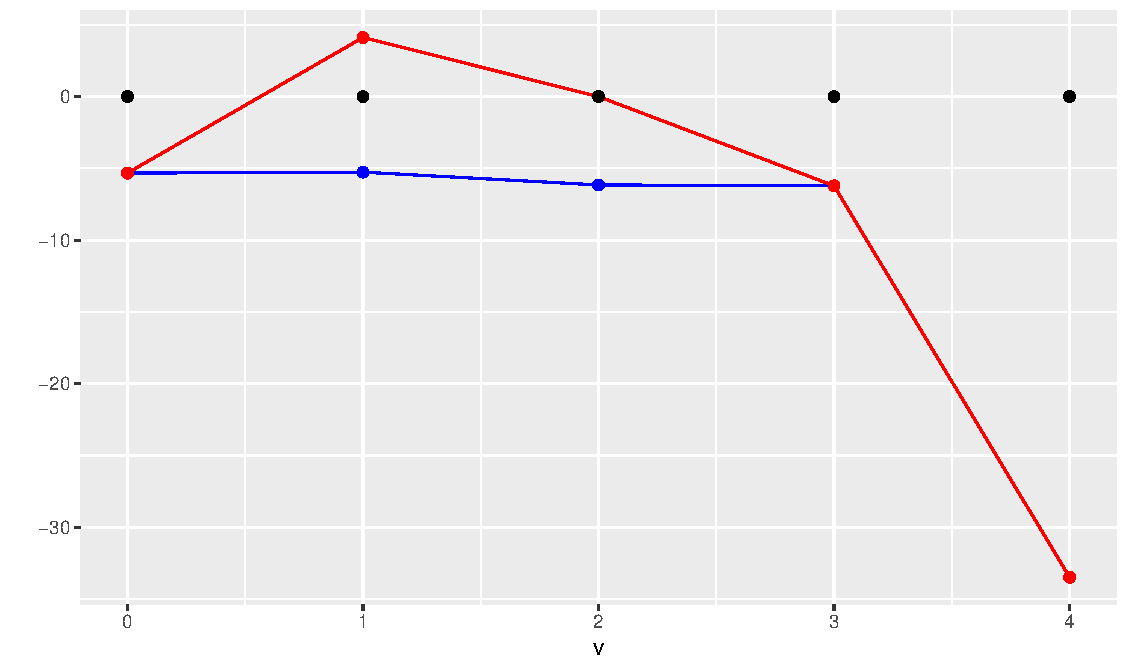
\includegraphics[scale=0.6]{plot1.pdf}
%\caption{}
%\label{fig:bounds}
\end{figure}

\newpage


\begin{table}[h!]
\centering
\begin{tabular}{cccccc}
\toprule
$v$ & 1 & 2 & 3 & 4 & 5\\
\midrule
$c_v(U)$ & -5.26 & 4.19 & 1.38 & -5.24 & -32.53\\
$c_v(L)$ & -5.26 & -5.06 & -4.93 & -5.24 & -32.53\\
\midrule
rejection & T & ? & ? & T & T\\
\bottomrule
\end{tabular}
\end{table}

However, if there is a column $\tilde{\mathbf{D}}_j$ ($j>1$) such that all the elements are non-positive, then also the following columns will be non-positive, and from that point on the upper critical value $c_v(U)$ will not increase. In particular, when $c_v(U)$  becomes negative, it will always remain negative, and thus all supersets from that size to $f$ will be rejected. Hence:
\begin{itemize}
\item we determine the column index $j$, if it exists;
\item we compute the lower bound up to column $j-1$ (size $|S|+j-2$), to check for non-rejections;
\item if needed, we continue by computing both bounds until $c_v(U)$ becomes negative. We know that higher sizes are all rejected;
\item finally, $c_v(U)$ is computed for columns from 1 to $j-1$, in order to determine indecisive sizes.
\end{itemize}
If at any point a non-rejection is found, the search stops.

In this case, $j=4$. The lower bounds up to size 3 are all negative, hence there are no non-rejections. 



\newpage
\paragraph{Branch and Bound method.} The first index, $i=1$, determines the branching rule:


\begin{table}[h!]
\centering
\begin{tabular}{c|ccccccc}
 & \multicolumn{3}{c}{remove} & & \multicolumn{3}{c}{keep}\\
 & \multicolumn{3}{c}{$S\subseteq V\subseteq F\setminus\{1\}$} & & \multicolumn{3}{c}{$S\cup\{1\}\subseteq V\subseteq F$}\\
\cline{2-4} \cline{6-8}
|S|+2 & $\{2,3,4\}$ & $\mathbf{\{2,3,5\}}$ & $\{3,4,5\}$ & & $\{1,2,3\}$ & $\{1,3,4\}$ & $\{1,3,5\}$ \\
|S|+1 & $\{2,3\}$ & $\{3,4\}$ & $\mathbf{\{3,5\}}$ & & & $\{1,3\}$ &  \\
\end{tabular}
\end{table}

In the "remove" branch, the lower bound remains the same, as the sum of the last $v$ columns of $M$ is not affected by the removal of the first column. However, the upper bound changes in both branches, as the elements corresponding to $i=1$ (in $I$) are removed.



\vspace{5mm}
\paragraph{To do.} Check common addenda between keep and remove.

\vspace{3mm}
Check the shape of the upper bound curve. Does it always decrease from some point on? (Such point being when a column of $D$ has all negative elements). If it is true, we can compute the points where the curve crosses zero: we automatically reject for all the sizes such that the curve is below zero.

Consider two vectors
\begin{align*}
&X=(x_1,\ldots,x_B)^\top\in\mathbb{R}^B  & Y=(y_1,\ldots,y_B)^\top\in[0,+\infty)^B
\end{align*}
as well as their difference $Z=X-Y$. Let $q_X$ and $q_Z$ be the quantiles of $X$ and $Z$, such that
\begin{align*}
&P(x_i\leq q_X)=1-\alpha  & P(z_i\leq q_Z)=1-\alpha .
\end{align*}
Since $z_i\leq x_i$ for each $i$, then $P(z_i\leq q_X)\geq P(x_i\leq q_X)=1-\alpha=P(z_i\leq q_Z)$. As a consequence, $q_X\geq q_Z$.

\vspace{3mm}
Check the behavior of different test statistics, e.g. harmonic mean p-value, Fisher combination etc.


\end{document}